\documentclass[10pt]{article}
\usepackage{parskip}
\usepackage[utf8]{inputenc}
\usepackage[left=2.00cm, right=2.00cm, top=2.00cm, bottom=2.00cm]{geometry}
\usepackage[spanish]{babel}
\usepackage{graphicx,subfig}
\usepackage{fancyhdr}
\graphicspath{{Imagenes/}}
\usepackage{enumerate} 
\usepackage{multicol}
\begin{document}


\pagestyle{fancy}
\cfoot{}


%Cabeceras
\rhead{Distribución de las cargas eléctricas}
\lhead{}

%Portada
\begin{titlepage}
	\newgeometry{
		left=25mm,
		right=25mm,
		top=5mm,
		bottom=30mm,
		headheight = 0 mm
	}

	\begin{figure}[t]
		\subfloat{
\includegraphics[width=0.15\textwidth]{Logo_IPN}}
		\hspace{0.6\textwidth}
		\subfloat{
\includegraphics[width=0.22\textwidth]{LogoEsime}}
	\end{figure}

	\centering
	{\bfseries\Huge Instituto Politécnico Nacional. \par}
	\vspace{1cm}
	{\scshape\Large Ingeniería en Comunicaciones y Electrónica. \par}
	\vspace{0.3cm}
	{\scshape\Large Laboratorio de Electricidad y Magnetismo.  \par}
	\vspace{1cm}
	{\scshape\Huge ECHALE TIERRA \par}
	\vspace{1cm}
	{\itshape\Large Distribución de las cargas eléctricas en los conductores. \par}
	{\Large 2CM13\par}
	\vfill
	{\Large Autores: \par}
	{\Large Daniela Elizabeth Pérez Vargas. \par}
	{\Large Jesús Martinez Amac. \par}
	{\Large José Emilio Hernández Huerta. \par}
	{\Large Nataly Bejarano Garduño..\par}
	{\Large Uriel Grimaldi Díaz.  \par}
	\vfill
	{\Large Abril 2023. \par}

\end{titlepage}

\tableofcontents
\newpage




\section{Resumen.}
Por medio de los materiales proporcionados en el laboratorio de la escuela, los alumnos realizaron experimentos con relacion a la distribucion de cargas en los conductores, siendo especificos realizaron estos experimentos con la ayuda de un generador Vander Graff, un electroscopio y diversos materiales más. Para llegar a tener las conclusiones necesarias para entender los conceptos basicos de electricidad y magnetismo.

\begin{multicols}{2}
\section{Objetivo.}
El alumno determinara mediante instrumentacion si un cuerpo esta cargado al igual de su polaridad, con las Experiencias de Cavendish y Franklin verificaran la carga electrica que se distrubuye en en la superficie exterior, razonaran el porque dentro de un conductor electrico hueco el campo electrico es nulo. Y para finalizar explicaran lo que sucede con el efecto puntas al realizar las experiencias del rejilete, la bujia y el mechon de cabello.

\section{Introducción.}
El ser humano es afectado por distintos fenomenos de la energia, entre ellos la electrizción de los cuerpos or los diferentes tipos inducción, frotamiento, contacto, al suceder este proceso en ocasiones existe una carga excesiva, esto sucede por la necesidad del objeto cargado por liberar la carga de más, es por ello que en esta liberación al contacto con el ser humano produce una reaccion que comunmente se le conoce como "toques", dejando en claro un concepto "la carga no se crea ni se transforma, solo se distribuye". 


\section{Marco teórico.}
La distribución de cargas eléctricas en los conductores está basado en la Ley de Coulomb, la cual establece que la fuerza de atracción o repulsión entre dos cargas eléctricas es directamente proporcional al producto de las cargas e inversamente proporcional al cuadrado de la distancia que las separa.

Cuando un conductor se carga eléctricamente, ya sea por contacto con otro conductor cargado o por la presencia de un campo eléctrico externo, las cargas eléctricas se distribuyen de manera uniforme en su superficie. Esto se debe a que, en un conductor, las cargas eléctricas se mueven libremente a través de su estructura cristalina, y tienden a distribuirse de manera tal que la densidad de carga sea uniforme en su superficie.

Además, la distribución de cargas en un conductor también está influenciada por la forma del conductor y la presencia de otros conductores cercanos. Por ejemplo, en un conductor esférico, las cargas eléctricas se distribuyen de manera uniforme en su superficie, mientras que en un conductor cilíndrico, las cargas tienden a acumularse en los extremos del cilindro.

La distribución de cargas en un conductor también puede ser afectada por la presencia de otros conductores cercanos. Cuando dos conductores están cerca uno del otro, las cargas eléctricas pueden redistribuirse de manera tal que la densidad de carga sea menor en las zonas cercanas al otro conductor, lo que se conoce como efecto pantalla.

En resumen, la distribución de cargas en un conductor está influenciada por la Ley de Coulomb, la forma del conductor y la presencia de otros conductores cercanos. En general, las cargas eléctricas tienden a distribuirse de manera uniforme en la superficie del conductor, y cualquier desviación de esta distribución puede ser explicada por los efectos de la geometría y la presencia de otros conductores cercanos.


\section{Descripción de materiales.}

 Generador de van der Graff: sirve para acumular gran cantidad de carga eléctrica dentro de su esfera hueca.
 
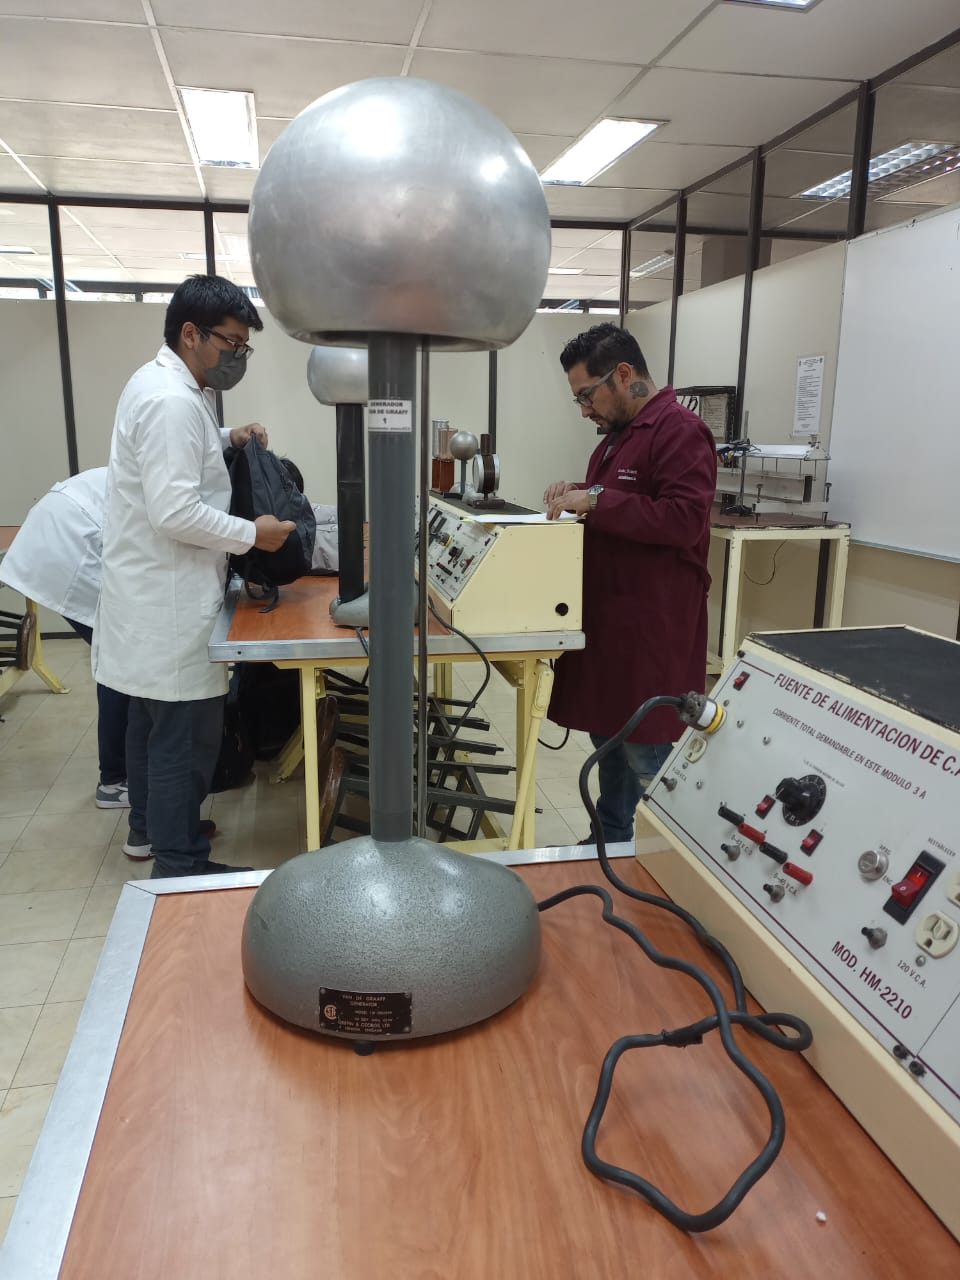
\includegraphics[width=0.1\textwidth]{Vander} 
	
	

Electroscopio: es un instrumento que se utiliza para saber si un cuerpo esta eléctricamente cargado. 

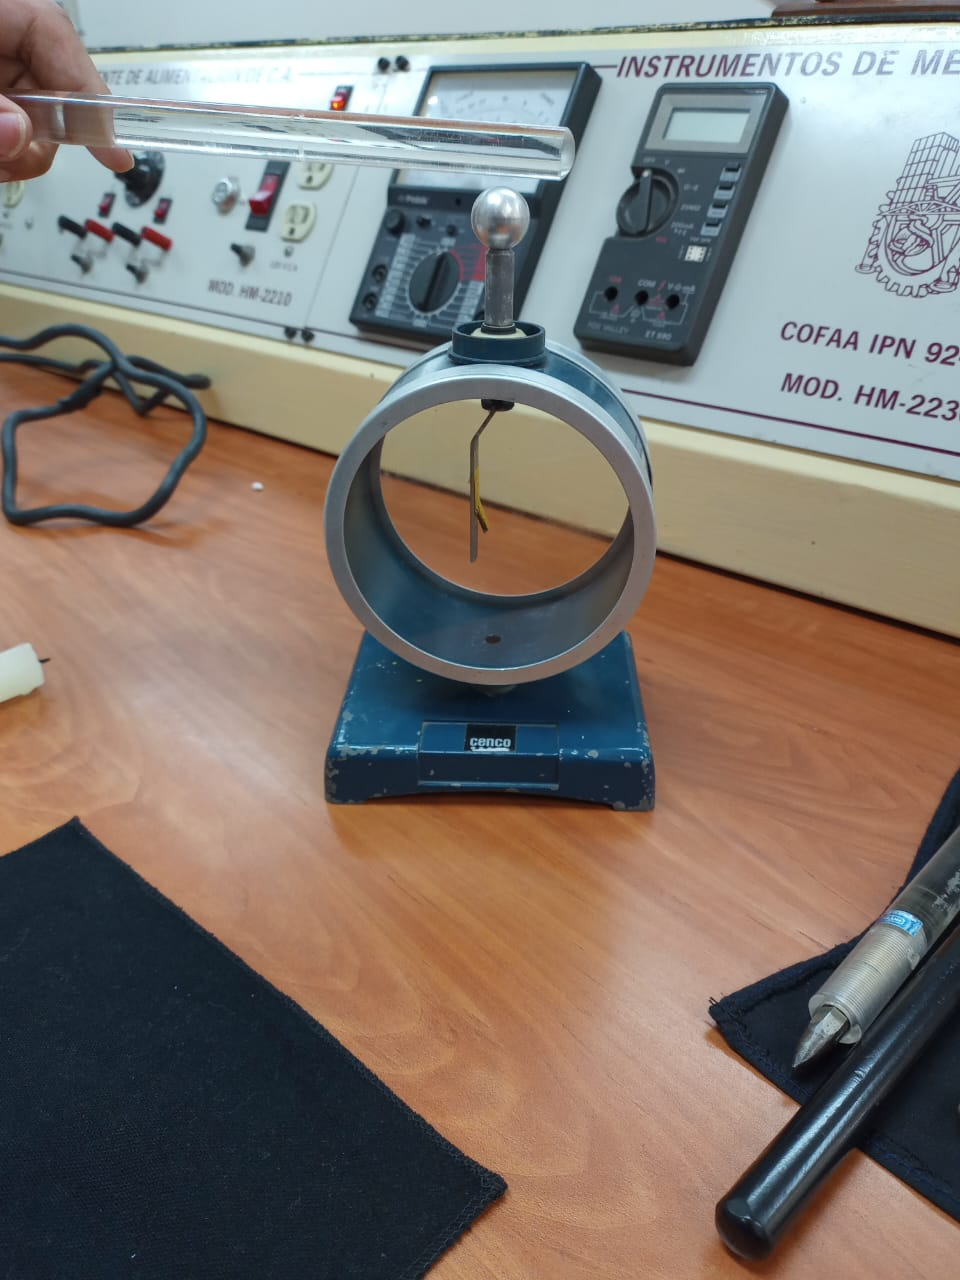
\includegraphics[width=0.1\textwidth]{Metro}

Mechón de cabello y Rehilete electrostático: 
Estos dos instrumentos fueron utilizados para ver la reacción de generador de Van der Graff en base a estos instrumentos y su electrización 

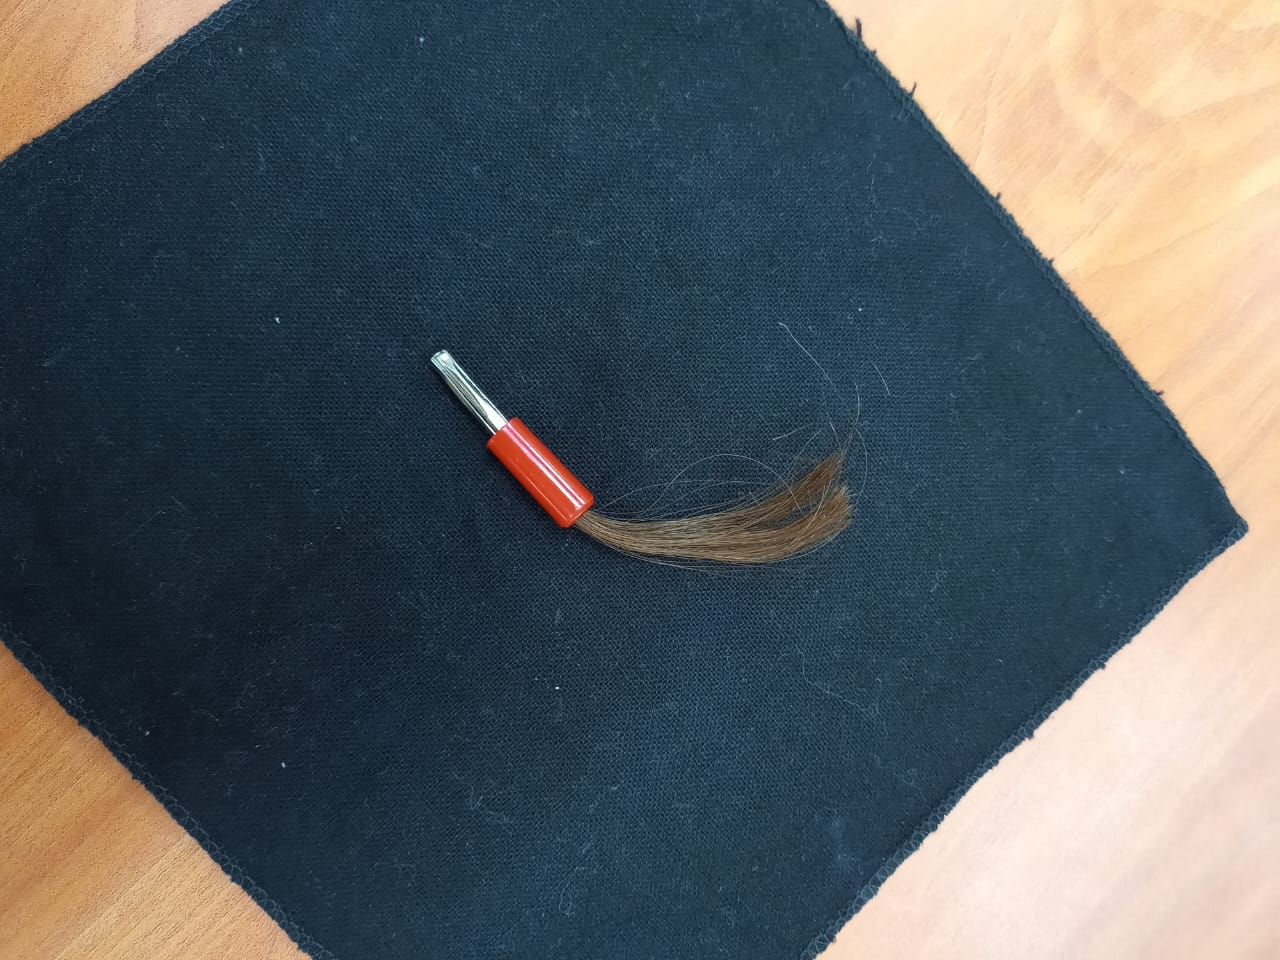
\includegraphics[width=0.1\textwidth]{Pelo}
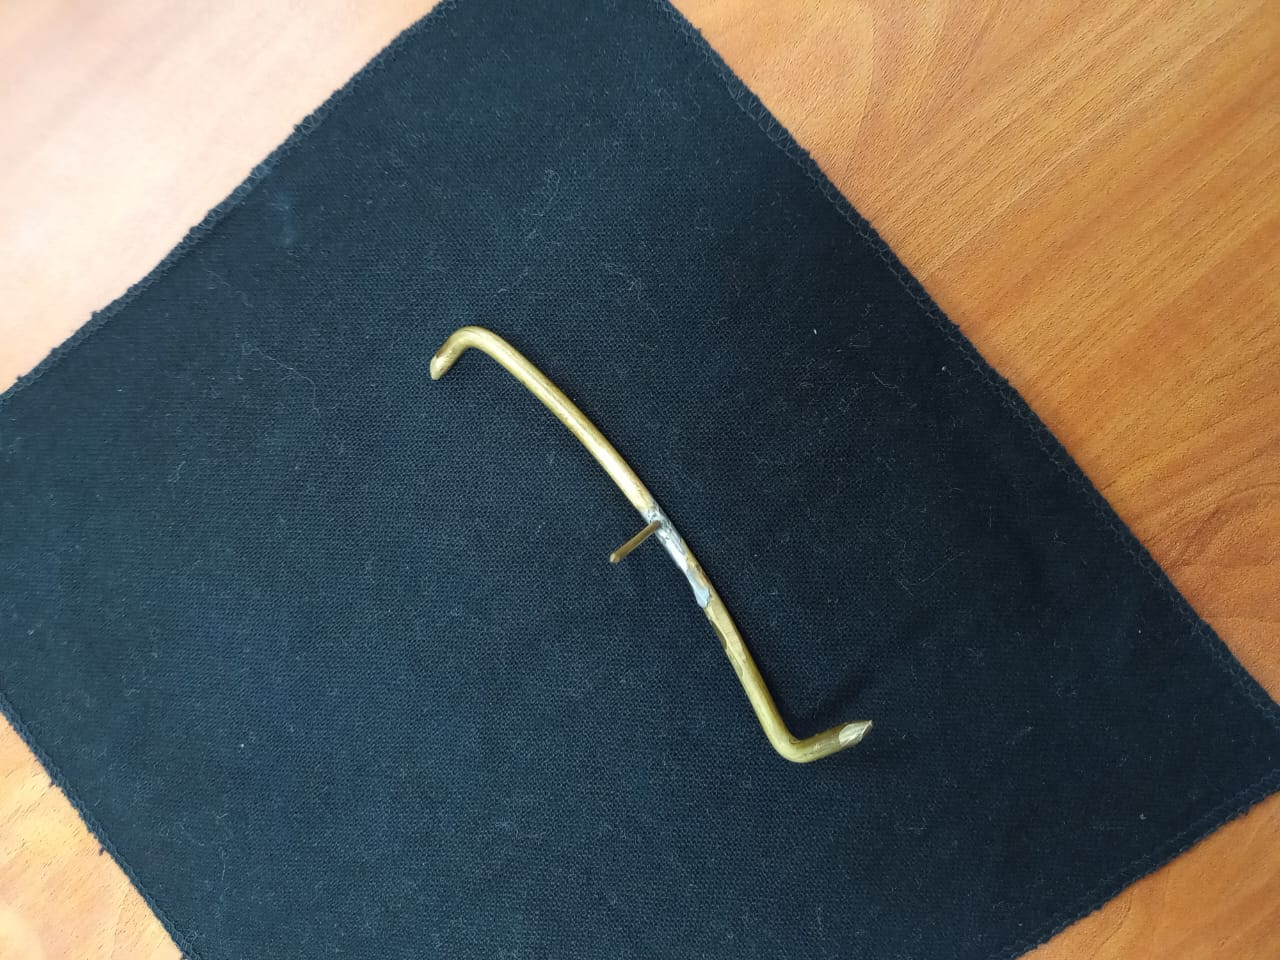
\includegraphics[width=0.1\textwidth]{Rehilete}


Banco aislado, copa de Faraday, recipiente de plástico con esferas de cripsota, esfera hueca, hemisferios de Cavendish
Estos materiales fueron utilizados para entender cómo se puede pasas la electrización de cuerpos con el generador y el electroscopio.

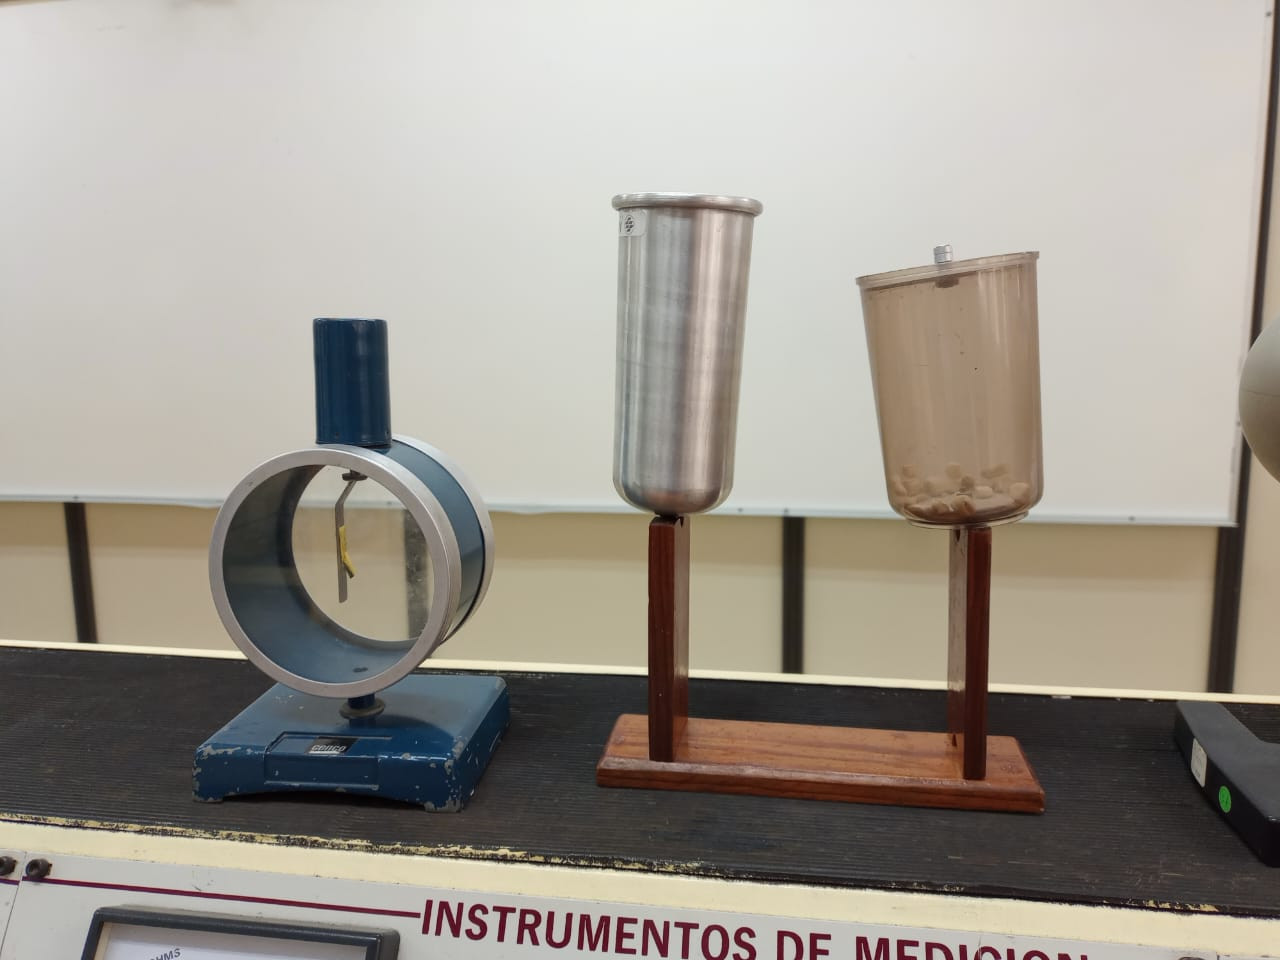
\includegraphics[width=0.1\textwidth]{copas}
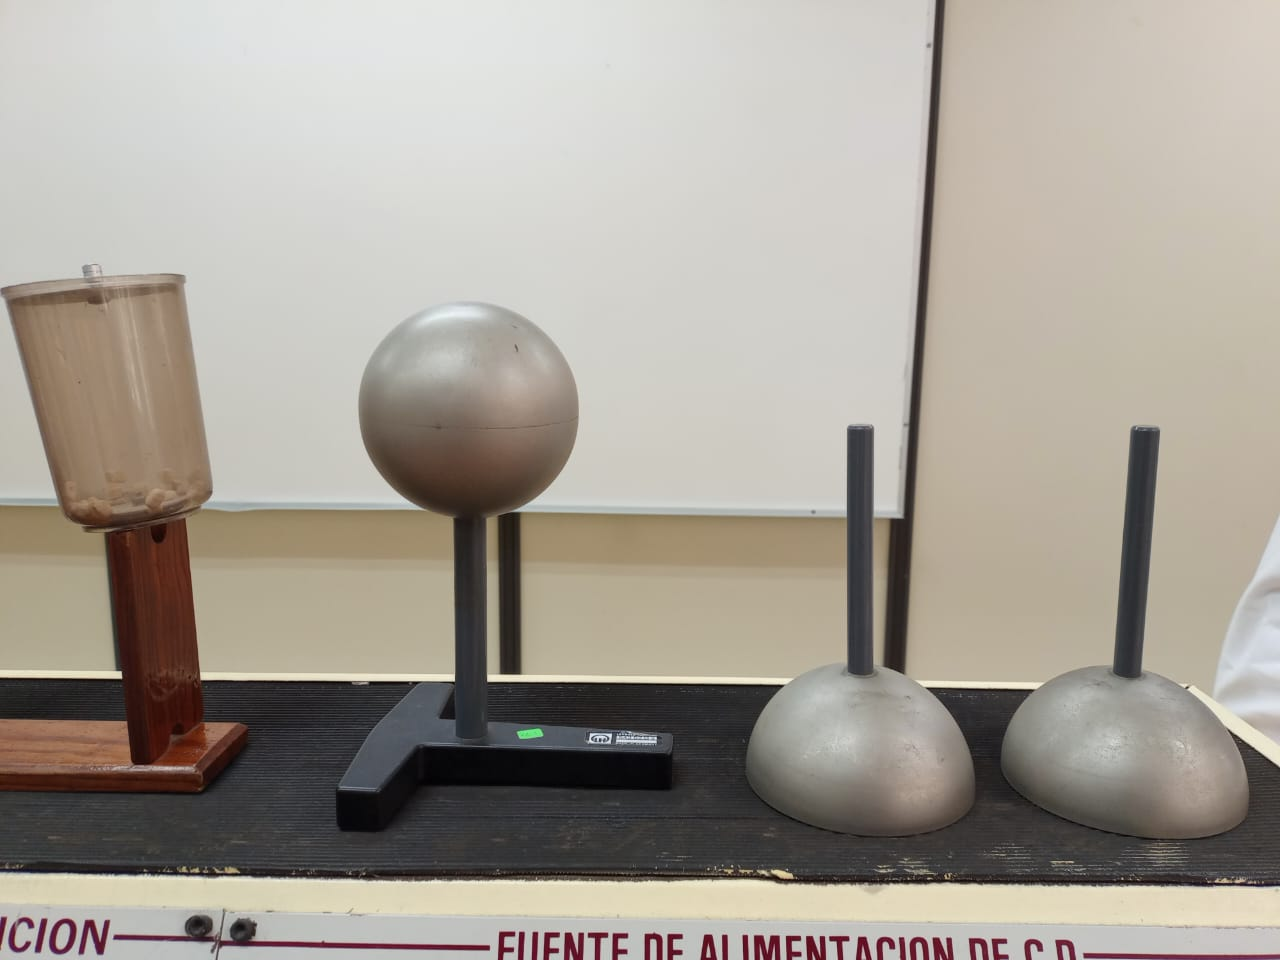
\includegraphics[width=0.1\textwidth]{bolas}

Barra de vidrio, Barra de poliestirena, Electrodo de prueba, paño de lana, paño de seda, punta de metal:
Estos instrumentos funcionaron para entender la electrización por contacto, por fricción y por inducción , a su vez el electrodo de prueba funciono para descargar los demás materiales que quedan con un poco de carga. 

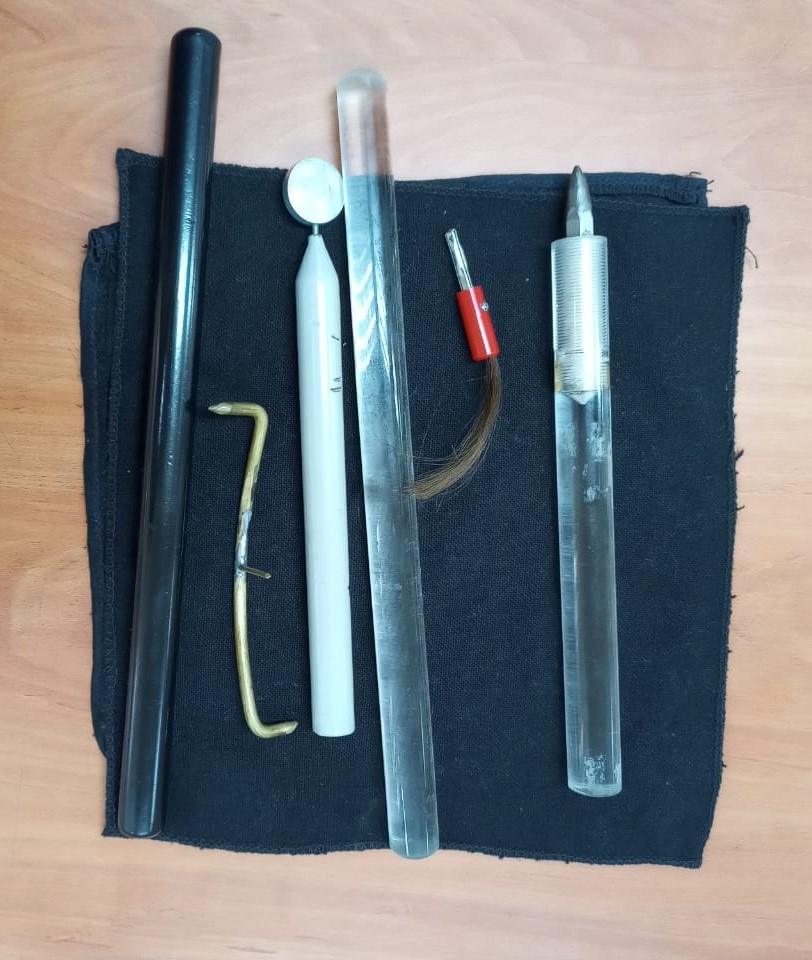
\includegraphics[width=0.1\textwidth]{Herramientas}
\section{Desarrollo experimental.}

\subsection{El electroscopio.}
Es un dispositivo formado por dos láminas ligeramente de aluminio, fijas a una varilla metálica, coronada por una esferilla de metál, la varilla se ajusta en un tapón aislador, tambien tiene dos ventanillas de cristal, esto permite ver en el interior del Electroscopio.

\begin{figure}[h]
\centering
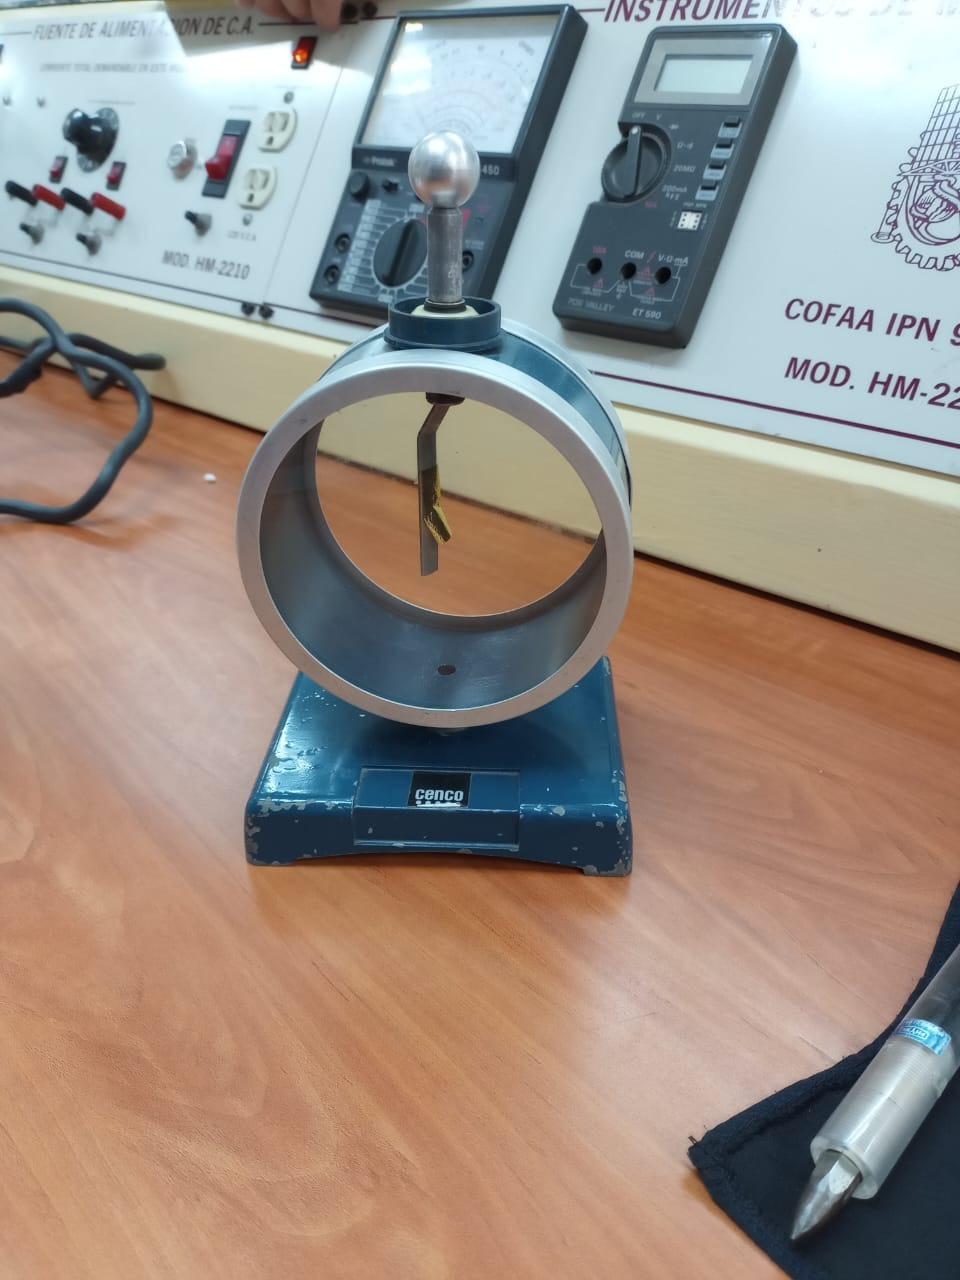
\includegraphics[scale=0.07]{p1}
\caption{Electroscopio de hojas}
\end{figure}

\subsubsection*{Procedimiento}
Acercamos a la esfera del electroscopio la barra de vidrio sin frotar, realizando lo anterior cargamos posterior mente por frotamiento la barra de vidrio acercandola hasta tocar la esfera del electroscopio.

\begin{figure}[h]
\centering
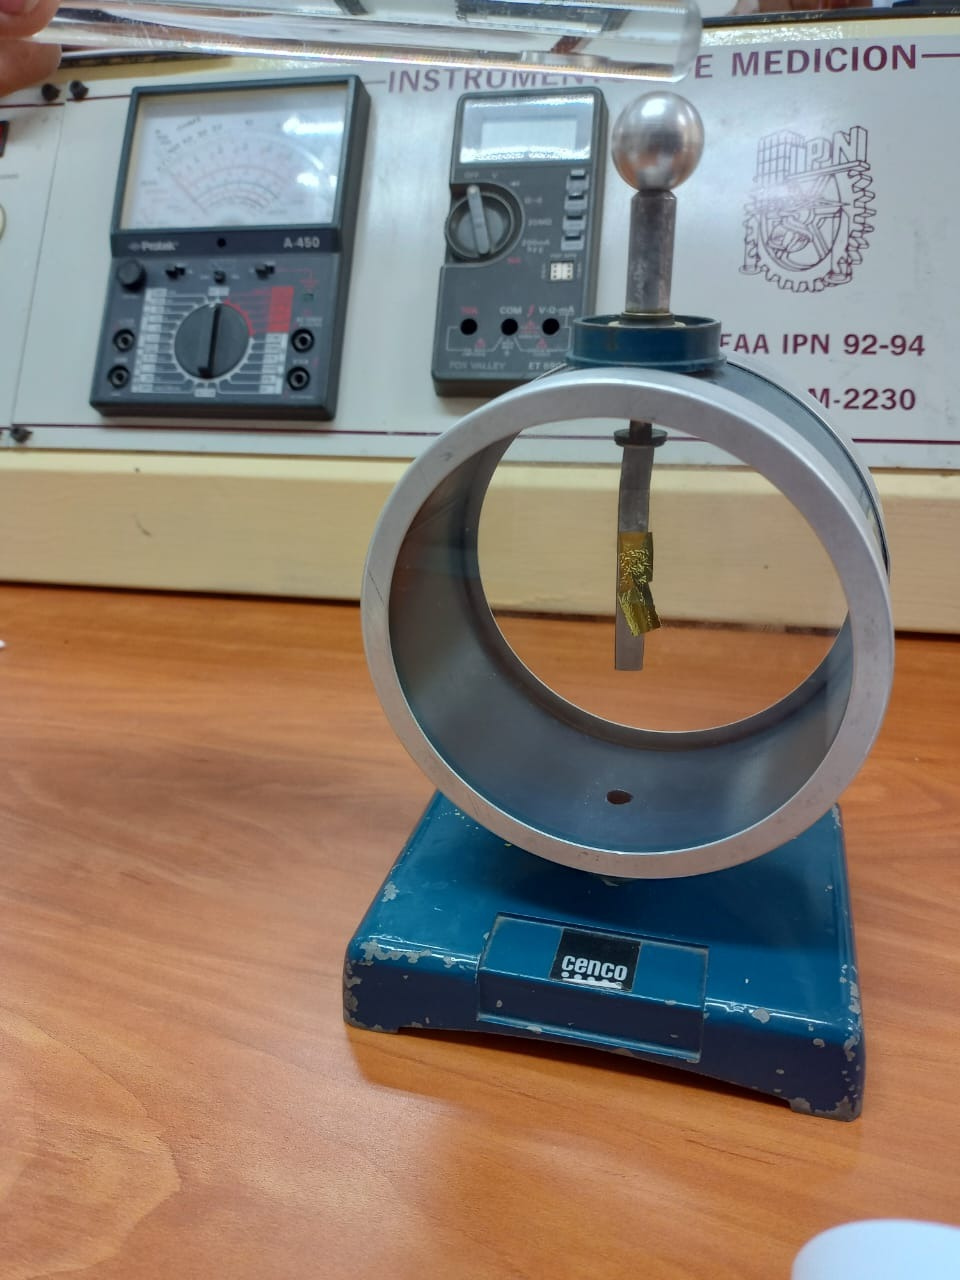
\includegraphics[scale=0.07]{p2}
\caption{Barra de vidrio sin carga.}
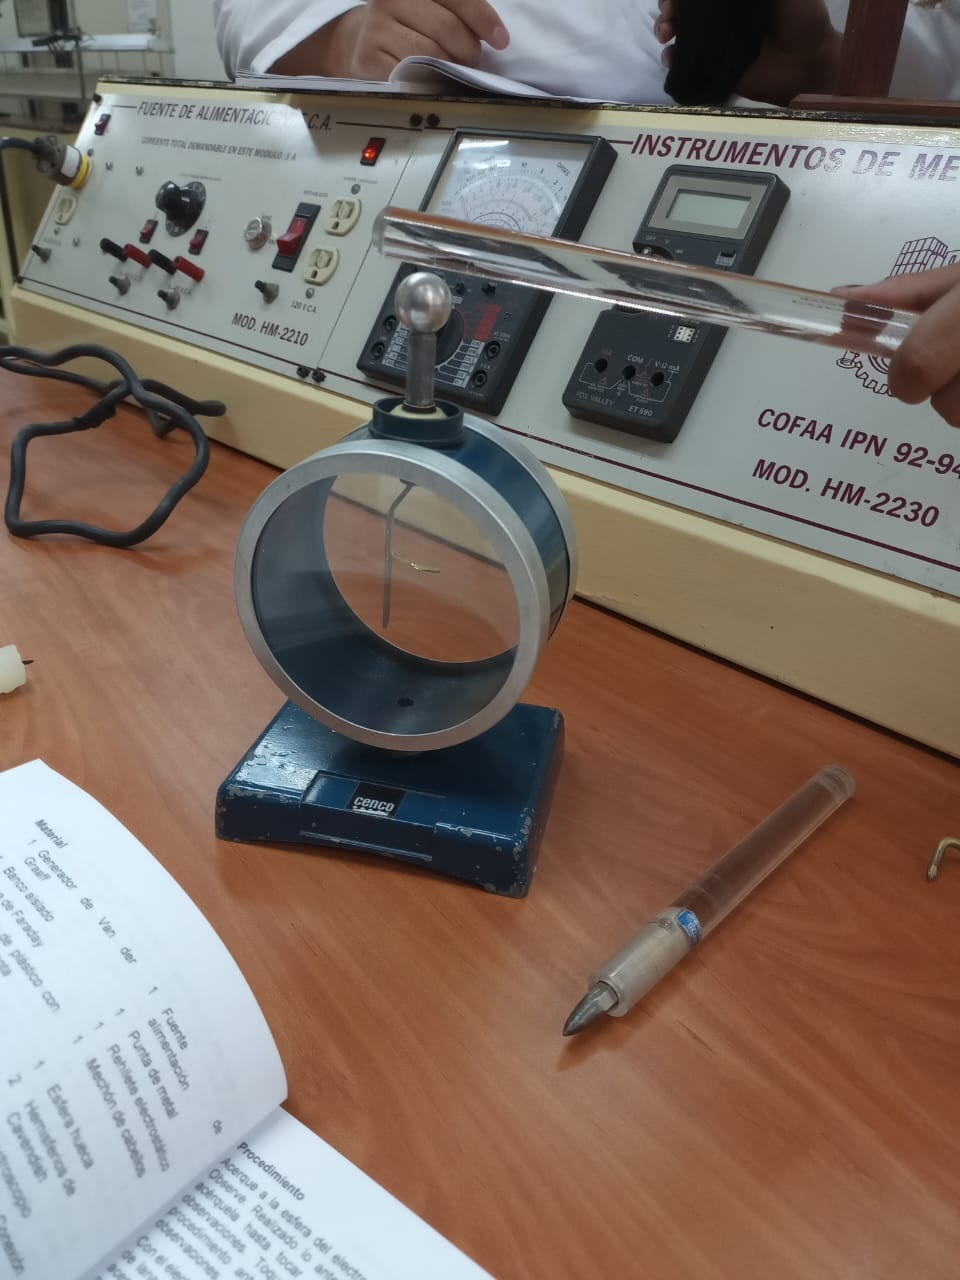
\includegraphics[scale=0.07]{p3}
\caption{Barra de vidrio con carga.}
\end{figure}

\subsubsection*{Conclusión}
Pudimos observar a la figura 2, que no pasa nada ya que la barra de vidrio notiene niguna carga electrica, sin en cambio la figura 3, pudimos observar el movimiento de las láminas de aluminio, ya que acercamos la barra de vidrio previamente cargada por la fricción, generando que al momento de acercar la barra de vidrio con el electroscopio ubiera generado un campo electrico.
\subsection{La experiencia de Cavendish.}
Montamos el arreglo experimental como se muestra en la figura 4.

\begin{figure}[h]
\centering
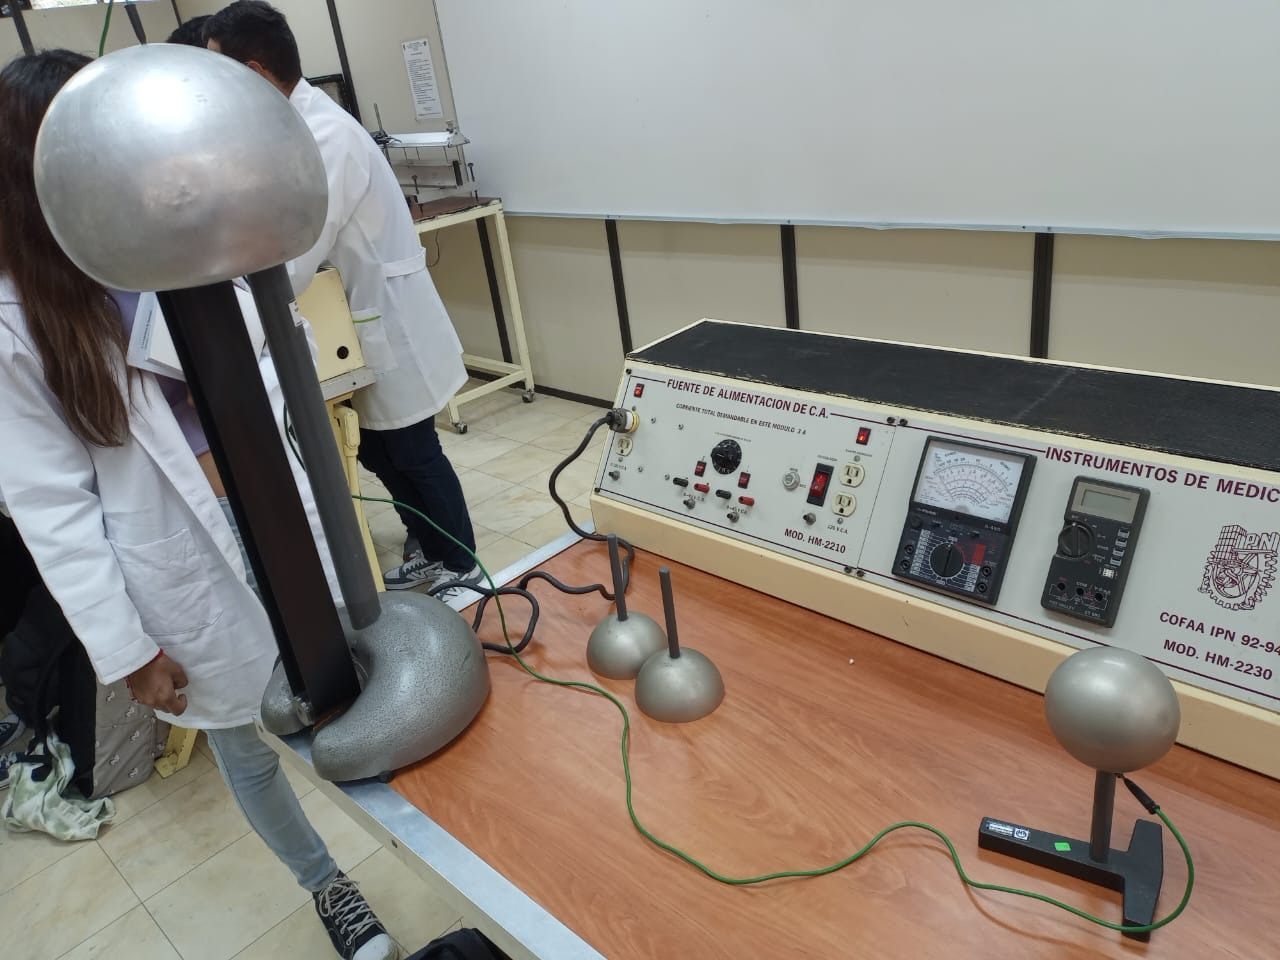
\includegraphics[scale=0.07]{p4}
\caption{}
\end{figure}

Una vez montado elarreglo experimental, pusimos a cargar la esfera metálica poniendo a funcionar el generador de Van de Graaff a velocidad minima durante un minuto aproximadamente y lo apagamos, una vez finalizado lo anterior desconectamos la esfera metálica hueca del generador, porcurando no tocar con las manos ni el generador ni la esfera, con la sonda de prueba tocamos cualquier punto de la superficie de la esfera y con la ayuda del electroscopio determinamos si esta cargada o no.

\begin{figure}[h]
\centering
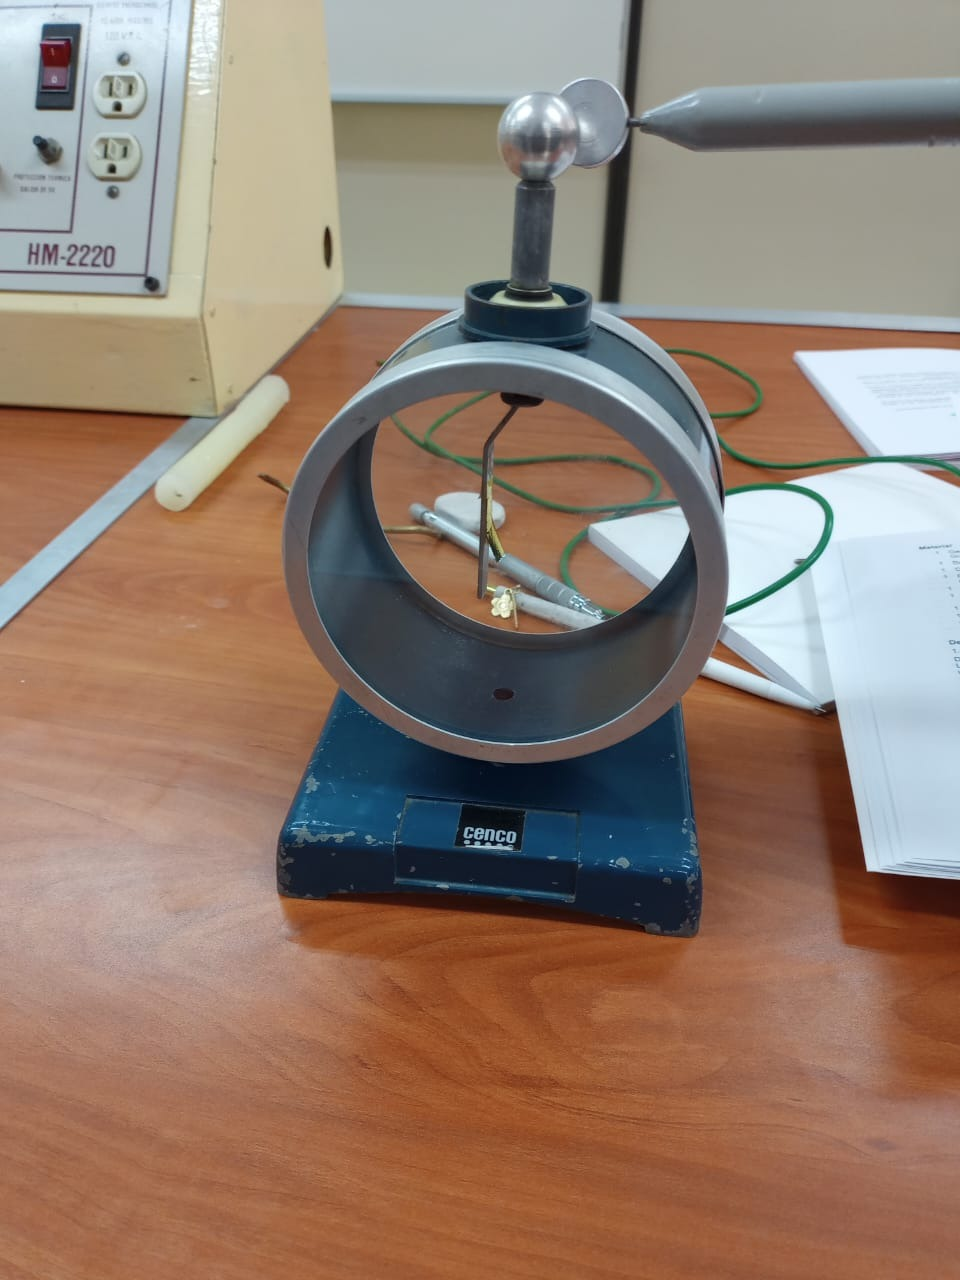
\includegraphics[scale=0.07]{p5}
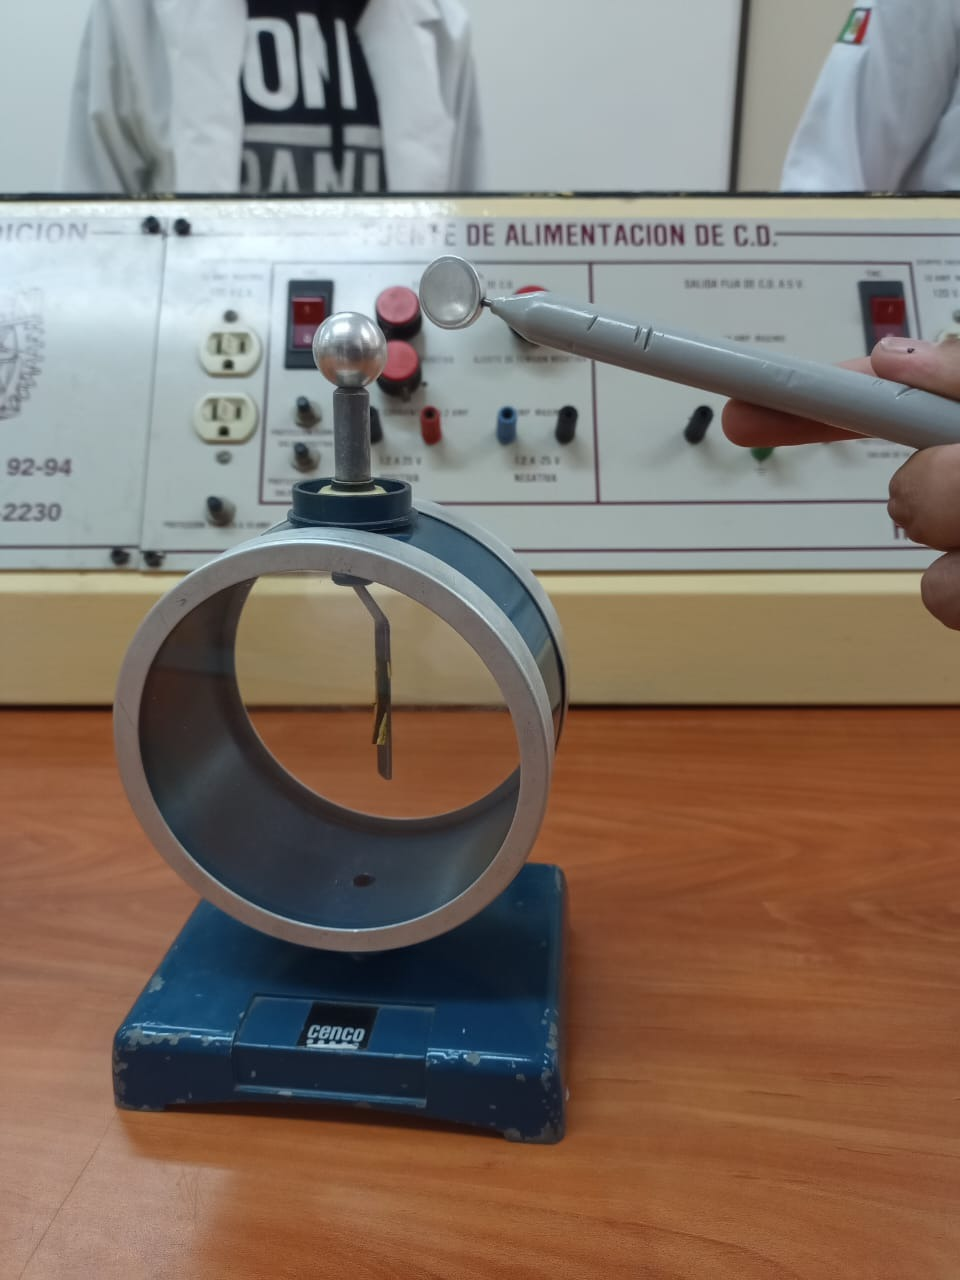
\includegraphics[scale=0.07]{p6}
\caption{Sonda de prueba con el electroscopio}
Nota: El electroscopio debe estar lo bastante alejado del generador de Van de Graaff para evitar su influencia.
\end{figure}

\subsubsection*{Conclusión}
Observamos que no logra pasar nada ya que no tiene niguna influensia de carga electrica respecto a la sonda de prueba.

\subsubsection*{Procedimiento}

Ahora tomamos los dos hemisferios metálicos descargados,cubrimos la esfera metálica con ellos,como se muestra en la figura 6, despues de unos segundos separamos ambos hemisferios y con la ayuda de la sonda de prueba y del electroscopio descargado, determinamos si existe una carga eléctrica en la esfera y en los emisferios.
\subsection{Experiencia de Franklin.}
Montamos el areglo experimental como se muestra en la figura 7.

\begin{figure}[h]
\centering
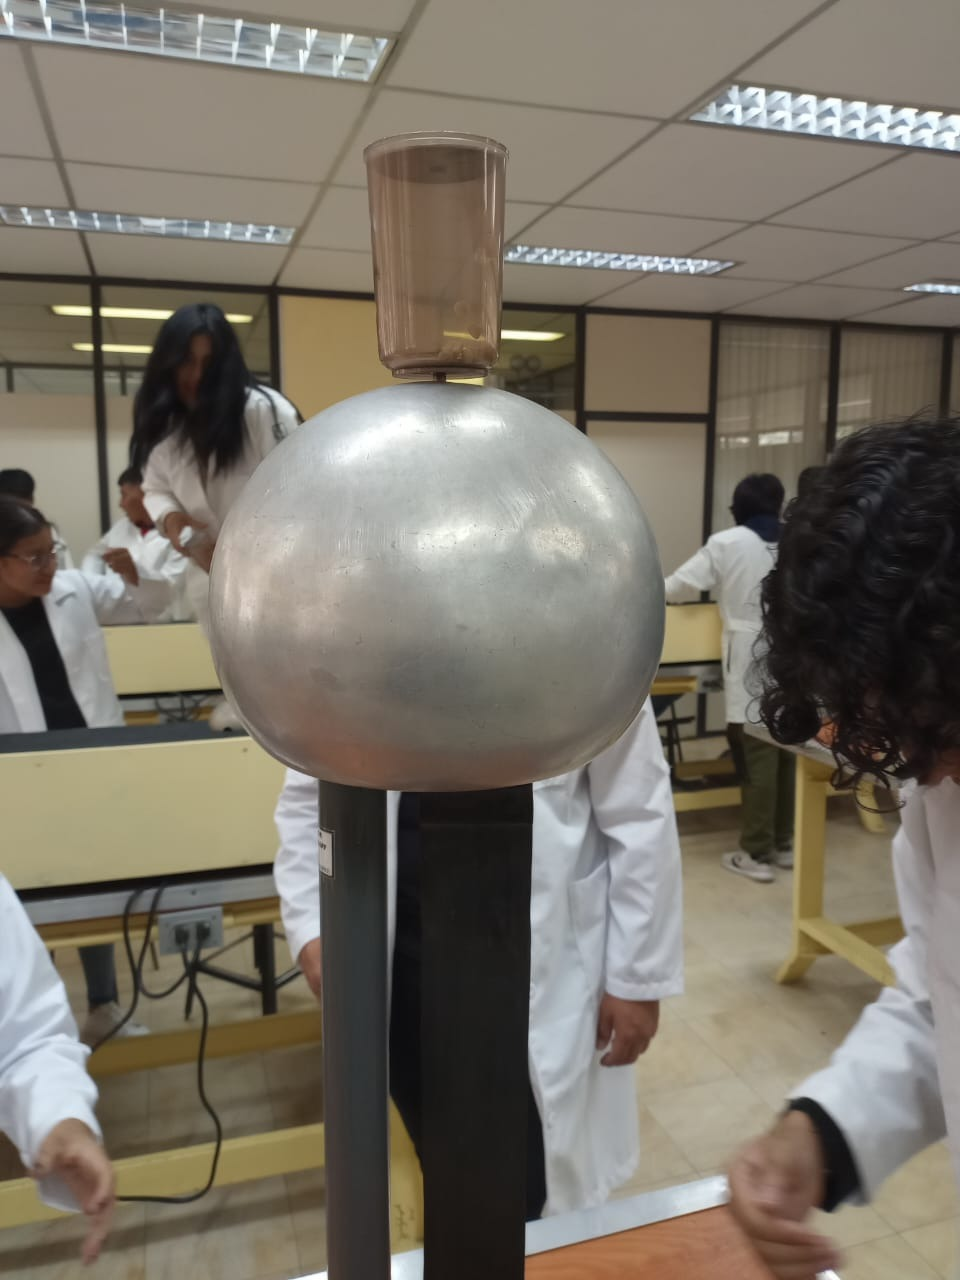
\includegraphics[scale=0.07]{p9}
\caption{Generador de Van de Graaf con las esferas de cripsote.}
\end{figure}

Una vez instalada la parte superior de la esfera colectora del Van de Graaff, previamente descargado el recipiente de plastico con base de metal, ponemos a funcionar a su minima velocidad durante algunos segundos, desconectamos el generador y lo descargamos.

\begin{figure}[h]
\centering
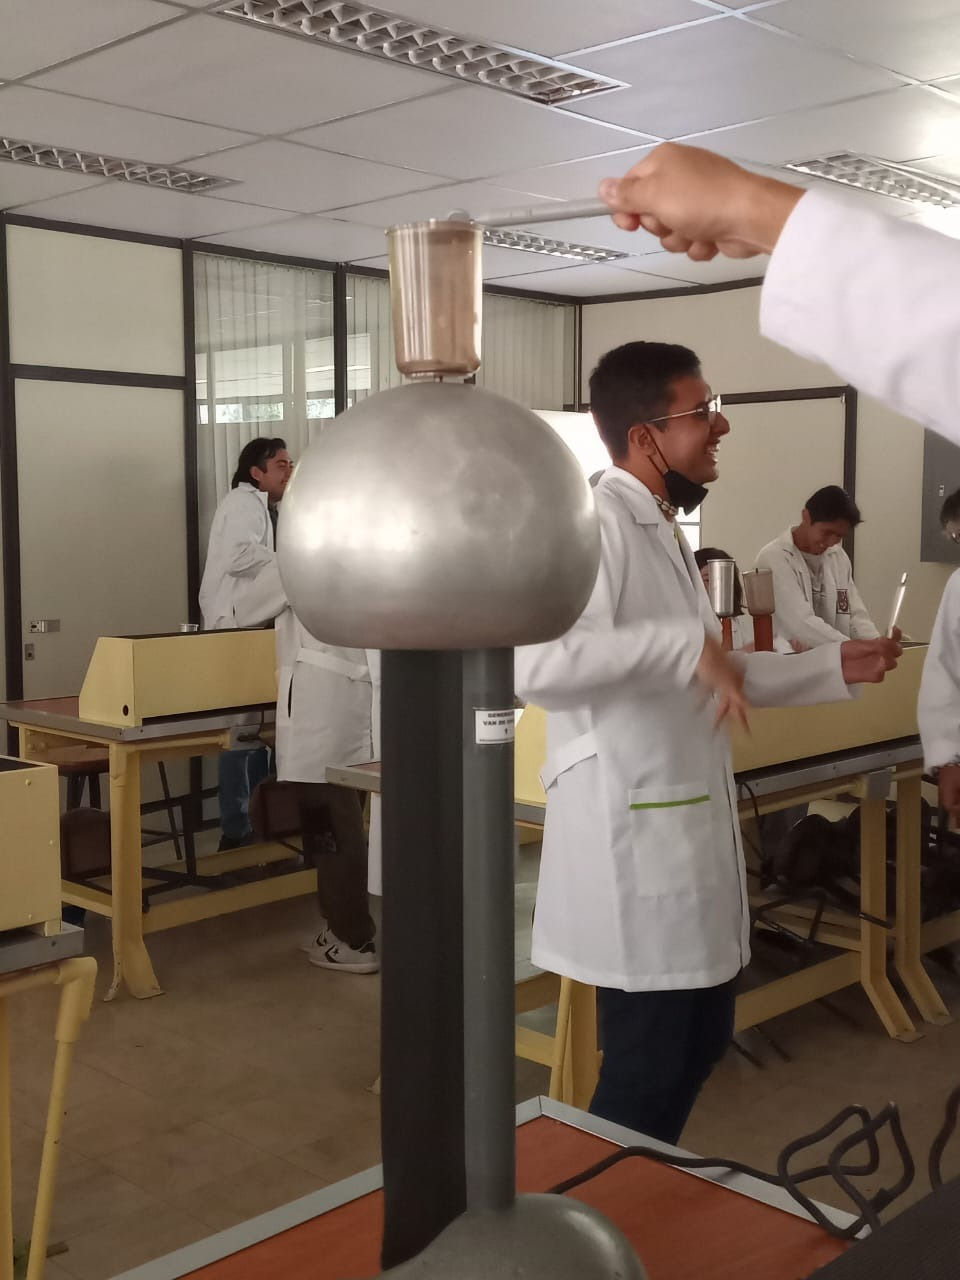
\includegraphics[scale=0.07]{p10}
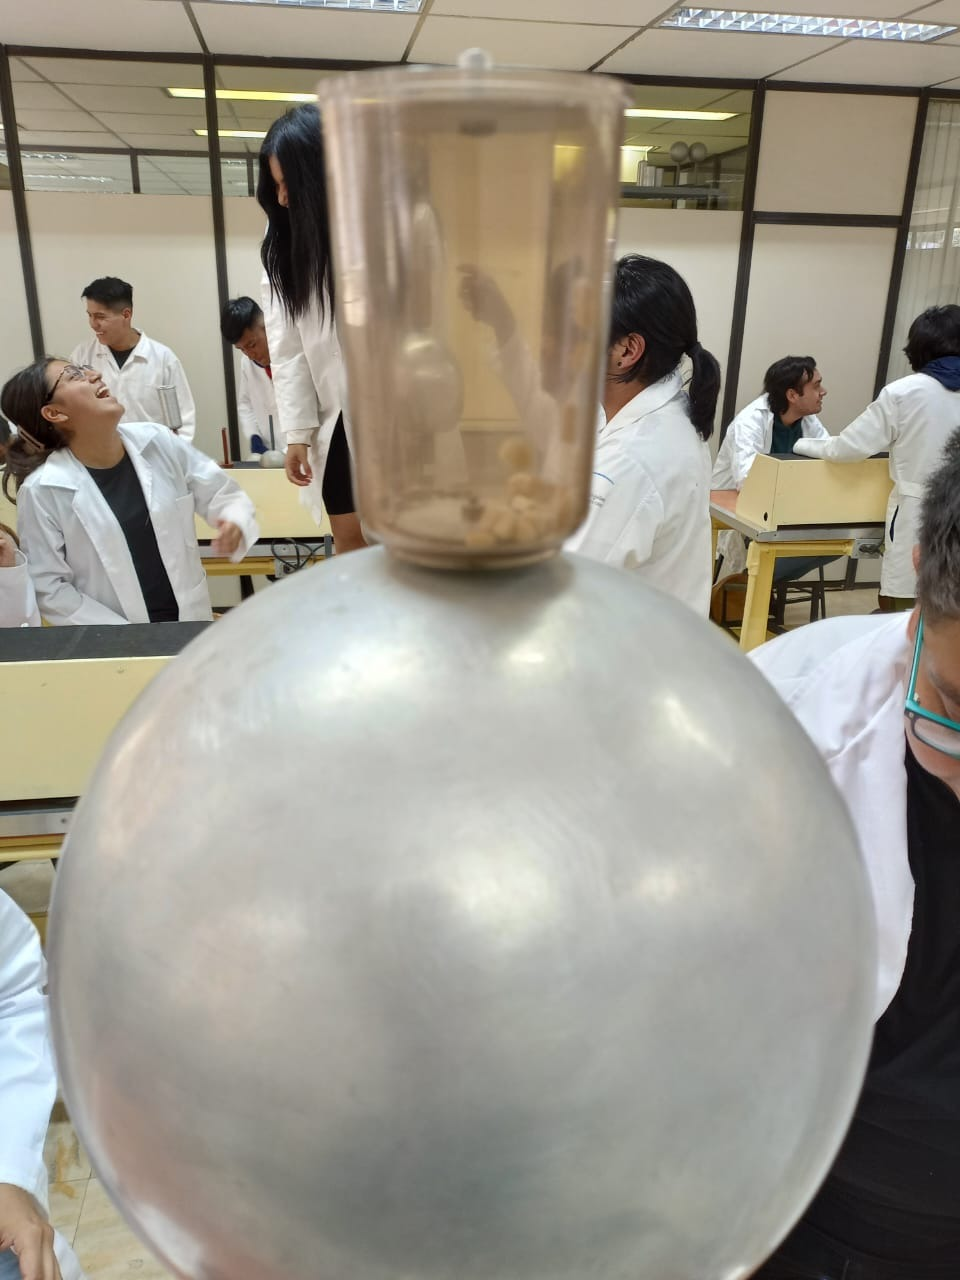
\includegraphics[scale=0.07]{p11}
\caption{Esferas de cripsote}
\end{figure}

\subsubsection*{Conclusión}
Observamos que en el areglo experimental de la figura 7, genero un campo electrico  grasias a la placa superior metálica del recipiente de plastico con las esferas de cripsote, asi pudiendo observar asimplevista con las esferas de cripsote que habia dos fuerzas electricas constantes, que era una negativa y una positiva.

\subsubsection*{Procedimiento}
Colocamos el cilindro de faraday en el generador de Van de Graaff como se muestra en la figura 9, ponemos a funcionar el generador a su minima velocidad durante algunos segundos.

\begin{figure}[h]
\centering
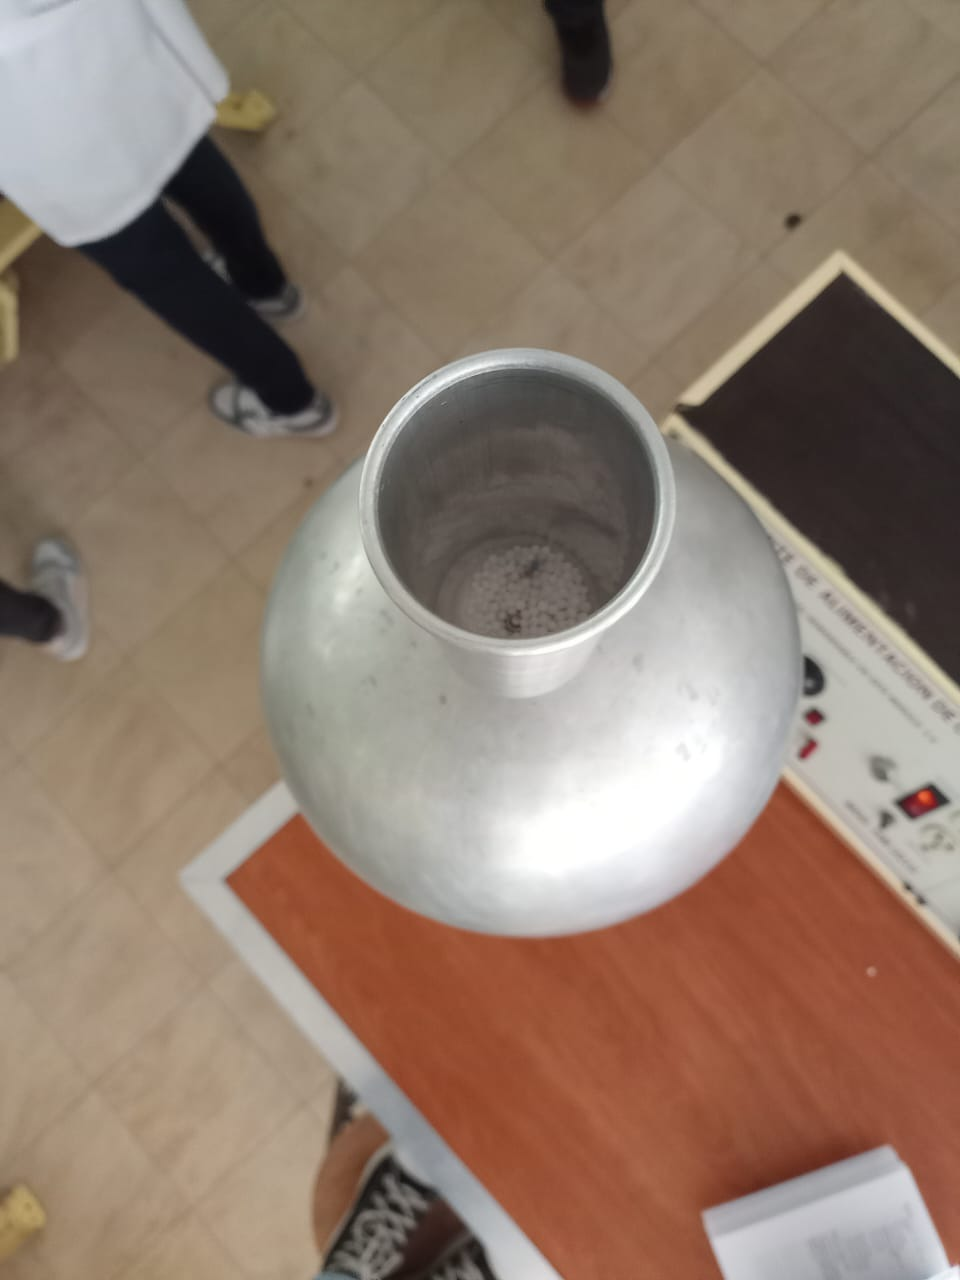
\includegraphics[scale=0.07]{p12}
\caption{Copa de faraday.}
\end{figure}

\subsubsection*{Conclusión}
Observamos que en el arreglo experimental de la figura 9, no pasa absolutamente nada ya que no hay una placa superior metalica que haga que genere un campo electrico.
\subsection{Pantalla eléctrica.}
Colocamos el capuchón metálico sobre el electroscopiio y lo conectamos a la esfera del generador como se muestra en la figura 10, pusimos a funcionar el generador a su minima velocidad.

\begin{figure}[h]
\centering
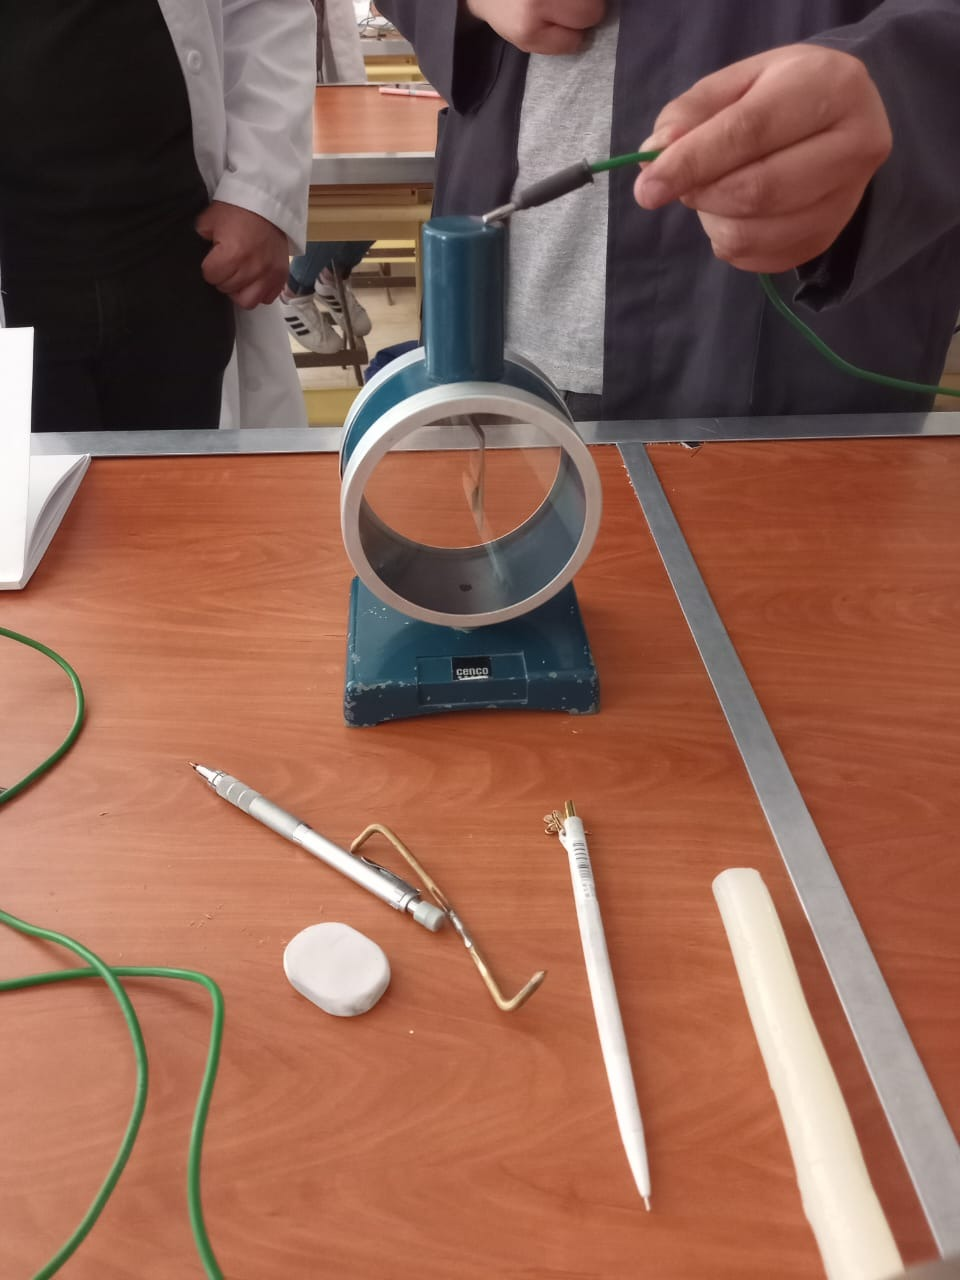
\includegraphics[scale=0.07]{p13}
\caption{Electroscopio con capuchón.}
Nota: Cuide que no haya arcos eléctricos entre el capuchón y el electroscopio.
\end{figure}
\subsection{Efecto de puntas.}
Instalamos el rehilete sobre la esfera colectora como se muestra en la figura 11, pusimos a funcionar el generador a su velocidad minima durante algunos minutos. 

\begin{figure}[h]
\centering
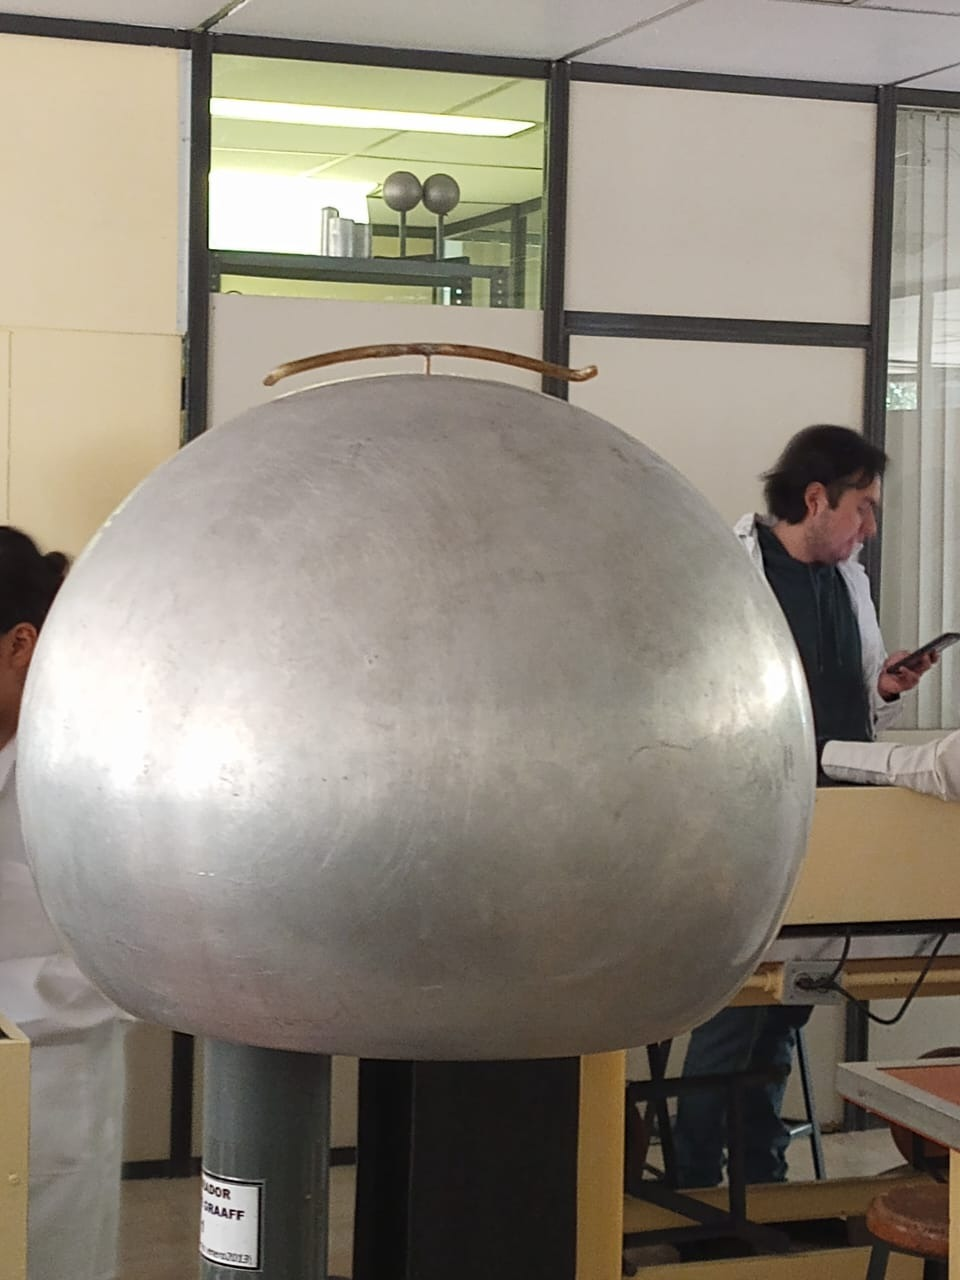
\includegraphics[scale=0.07]{p14}
\caption{Rehilete electrostático.}
\end{figure}

\subsubsection{Rehilete electrostático.}

\subsubsection{Mechón de cabellos.}
Descargamos el generador de Van de Graaff, quitando el rehilete y en su lugar pusimos el mechón de cabellos, pusimos a funcionar el genrador a una velocidad media durante un minuto.

\begin{figure}[h]
\centering
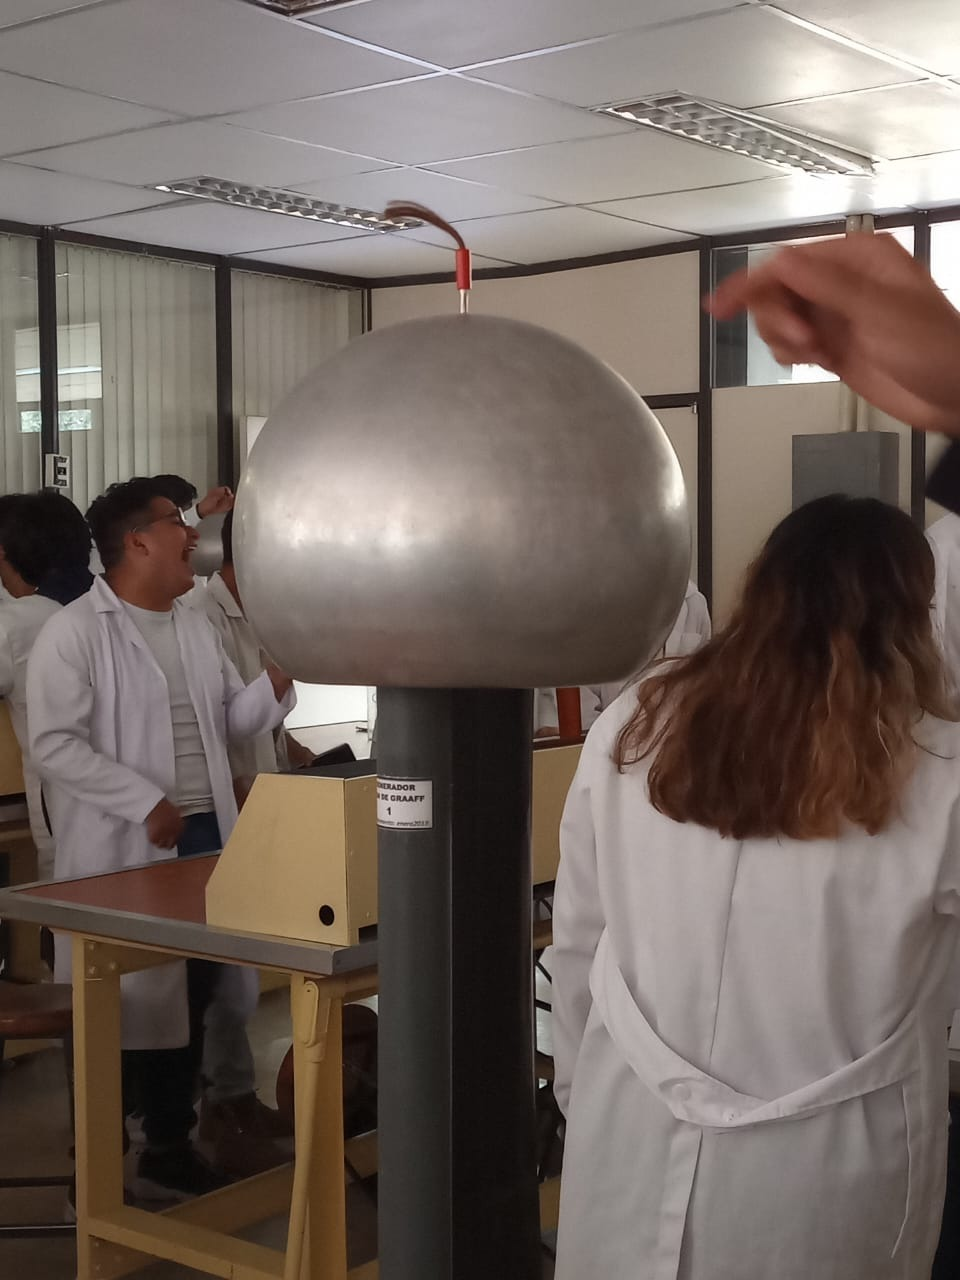
\includegraphics[scale=0.07]{p15}
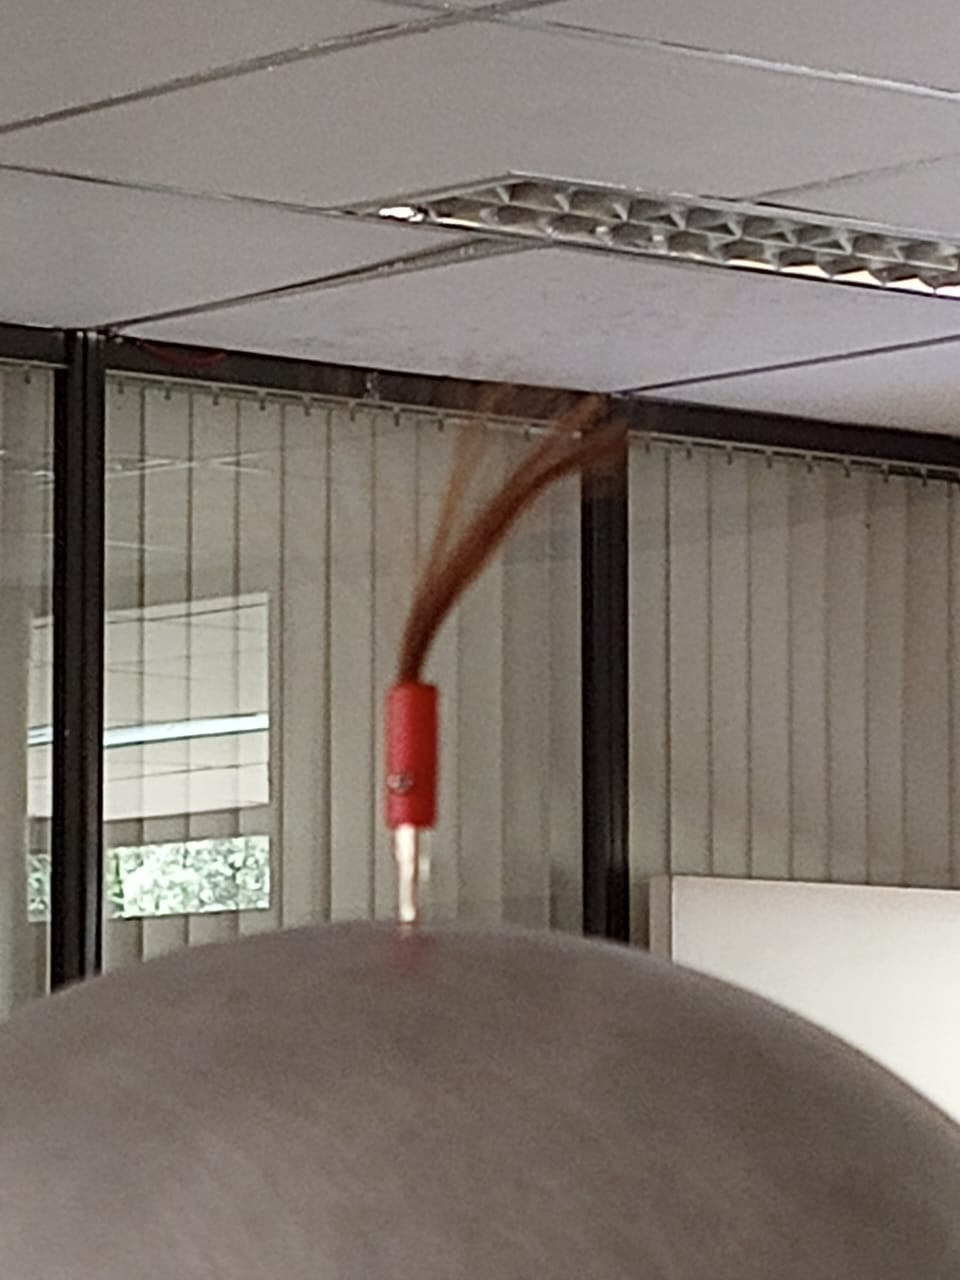
\includegraphics[scale=0.07]{p16}
\caption{Mechón de cabellos.}
\end{figure}
\subsubsection{Experiencia de la vela.}
Montamos previamente el arreglo experimental como se muestra en la figura 13, encendimos la vela y pusimos a funcionar el generador, acercamos la la flama de la vela a la punta metálica.

\begin{figure}[h]
\centering
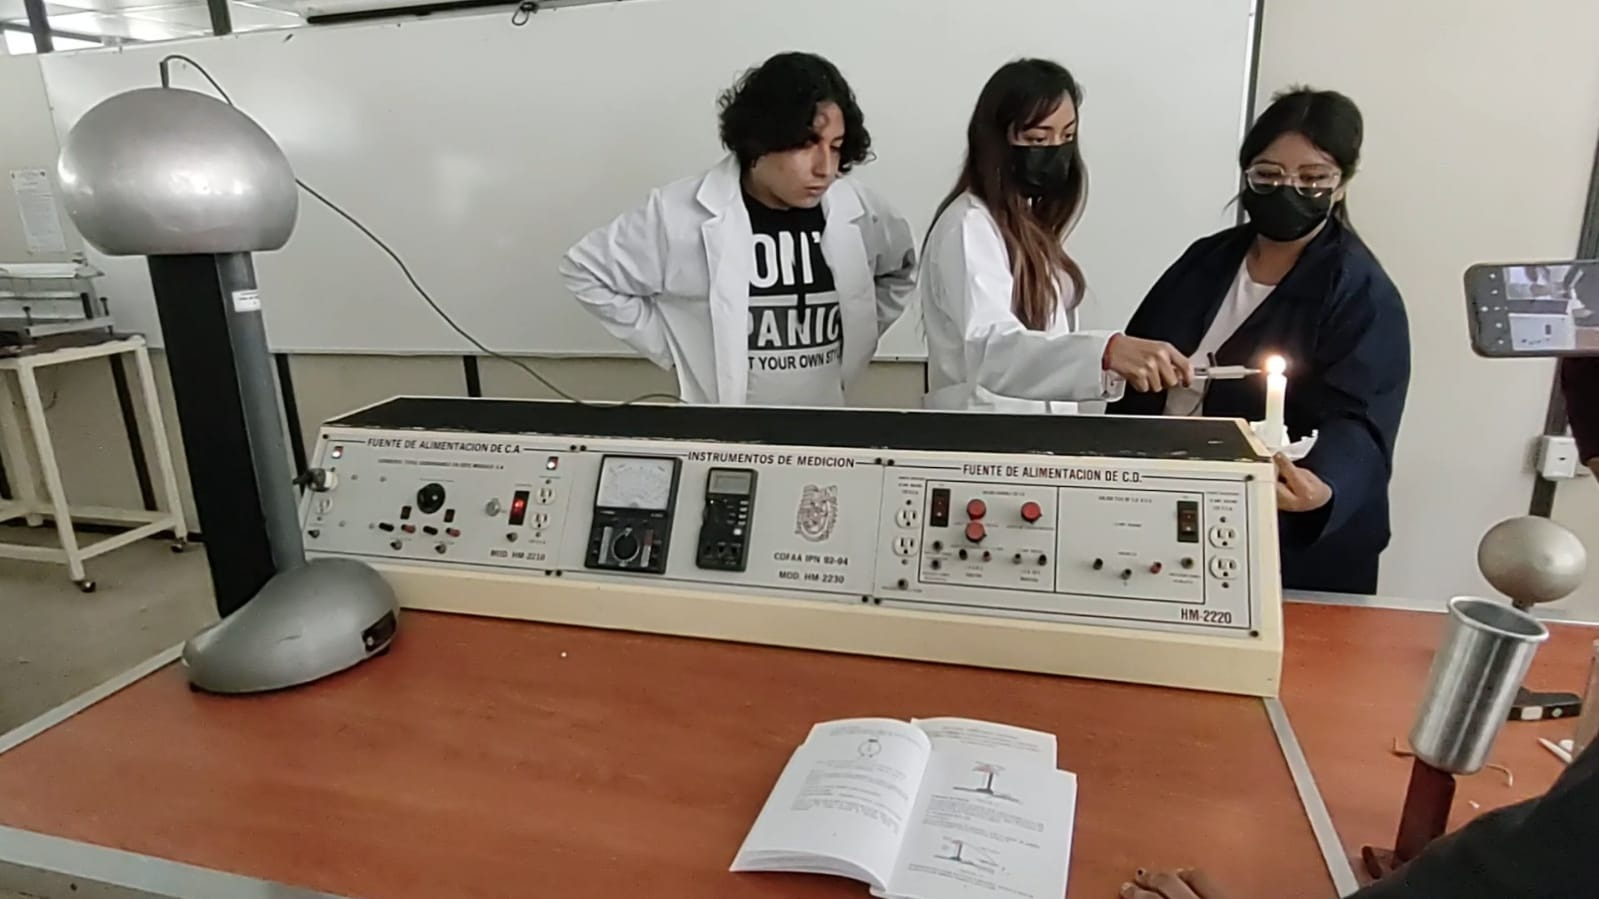
\includegraphics[scale=0.07]{p17}
\caption{Experiencia vela.}
\end{figure}

\section{Análisis y resultados.}

\section{Discución.}
Los procesos dados durante la practica son resultados de una serie de acontesimientos y teorias fisicas tales como electrostática, la conductividad, la Ley de Gauss, la densidad superficial de una carga, y conceptos como la jaula de Faraday.Lo cual la suma de todo esto genera que el electroscopio se muevan las pequeñas bolas dentro de los recipientes al igual que estos mismos principios son aplicados en el generador de Vander Graff. 

\section{Conclusiones.}
\subsection{José Emilio Hernández Huerta}
La practica introduce conceptos nuevos los cuales desonocia por completo al igual que nuevas experiencias a la hora de interactuar con el equipo del laboratorio demostrando como el cuerpo humano es un claro conductor al igual que entre mas superficie de contacto alla las cargas se distribuiran de mejor forma esto lo pude notar claramente al poner la lengua cerca del generador de Vander Graff. Pero esto es solo un pequeño acercamiento a lo que nos ofrece el curso, y todo el camino que nos falta pues en algunas practicas nuestras mediciones y observaciones fueron algo erroneas pues haciamos mal los experimentos, siendo que esto influya de manera negativa en nuestro aprendizaje y en nuestros reportes. En sintesis necesitamos mejorar nuestro metodologia de trabajo, aumentar nuestras horas de estudio para comprender mejor el tema y seguir adelante.
\subsection{Jesus Martinez Amac}
La practica consta en la distribución de cargas electricas en los conductores, pudimos observar las cargas electricas que destribuyen la presencia de los campos eléctricosexternos, podemos observar la distrubución de cargas eléctricas en un conductor  que puede afectar la forma en que interactua con otros conductores y campos eléctricos. Lo mas interesante para mi fue el experimento del rehilete con el generador de Van der Graaff, ya que pudimos observar una fuerza centripeta constant, haciendo girar el rehilete a favor de las manecillas del reloj.
\subsection{Nataly Garduño Bejarano}
La distribución de carga electrica se da mejor entre cuerpos electricamente cargados estando cerca que de lejos, es por ello que se involucra la distribución de carga. Así mismo, al usar el Generador de Vann der Graaff me percate que al existir un exceso de carga está busca liberarse de laguna manera, y por eso sentimos "toques". Por lo tanto, la energía no se crea ni se transforma, solo se distribuye. 
\subsection{Perez Vargas Daniela Elizabeth}
En la practica de laboratorio de distribucion de cargas electricas en los conductores, se pueden observar varios fenomenos interesantes, como la forma en que las cargas electricas se distribuyen en los conductores en funcion de su geometria y la presencia de campos electricos. En general se puede concluir que en un conductor de equilibrio electrostatico, las cargas electricas se distribuyen de manera uniforme en la superficie del conductor. Ademas la distribucion de las cargas electricas en un conductor puede afectar la forma en que interactua con otros conductores y campos electricos. 

\end{multicols}
\newpage
\clearpage
\begin{thebibliography}{0}
	\bibitem{}[Escamilla, E.(2017).Distribución de cargas eléctricas en los conductores.]
	www.academia.edu.
\end{thebibliography}

\end{document}

